\chapter{Optimizing fanout queries}

While we are focused mostly on the performance of reading queries, writes are one of the graph database's main purposes (as opposed to the more analytical types of systems).  Also, the kinds of techniques considered do not aim to improve reads at the cost of writes. So we do not  techniques that make writing more expensive.

\section{Optimizing fanout queries with two tier hashing}
\label{section:optfanout}
The main original contribution in this thesis is the idea, that for fanoutq queries, it pays to treat heavy degree vertices different from light degree ones.  There are two factors in play here, one is,  

1) in general, the system users benefit from reducing the variance in latency across calls (which reflects an underlying variance in degree) by making it more predictable. 

% we are talking about latency for a single operation (not for latency of several ones)

2) some latencies are simply too large to be acceptable %copy back of the envelope showing this
and the problem will keep getting worse.  An important feature of a service like twitter is the real-time feel it gives its users. It is undesirable to  becomes notable that some users receive tweets much before others. This also implies more complicated design within the rest of the system, as application logic demands no user sees a reply to a tweet before receving the tweet first.  Hence, extra work is done at different layers to hold on to tweets that cannot be delivered yet, 

This property is present in many naturally arising relations. eg. social networks etc.

This feature comes at the cost of complexity in the sharding mechanism. In fact, since there is no relation between the user id and whether it has a large degree, it is necessary to introduce lookup tables for this purpose. Luckily, we can use the graph property that  the degree is very skewed against itself: we only need to remember very few. 

%todo add another back of the envelope

This condition is helpful it would not be less plausible with a graph where there are two equally large classes of nodes to have a table for half those cases. in that case, though, we can do something such as cacheing, in case access patterns show some kind of skew. %complexity problems related to look

%(actually it would be interesting to analyze how cacheing relates to this, and maybe propose a solution based on it. Cacheing depends on skewedness in access patterns (ie acesess are only like to a few places), but cacheing policies can normally adapt online to handle distributions that change over time, as long as they remain skewed. Also, cacheing when the requests have a fanout.

For a given fanout size, there is an optimal number of partitions with respect to latency. For throughput, the optimal is probably  closer to 1.


The two main factors potentially afecting latency are 1) variability in network communication: the more nodes we request data from, the more likely
at least one will lag, affecting the performance of the whole operation 2) the more nodes we have, the more parallelism there is in reading.

\subsection{The cost of parallel requests}
Whenever we parallelize calls we reduce the work done at each node, but add the overhead of making more calls. If the calls are all made in a sequence (but without waiting for the previous to return in order to start the next), then we still have a cost linear in the number of nodes involved, with a smaller constant.    This overhead can be controlled by making a tree of calls (where a the calls themselves are organized in parallel), reducing this overhead to a $\lg{n}$ factor.  Nevertheless, there is an extra cost to making more calls. Each call made over a network has a natural, random, variability in latency. Since ultimately we need to wait for each of the parallel calls to finish, then we need to wait for the worst case of $n$. As $n$ increases, the latencies at each percentile level increase also. The exact way in which they increase depends on the original distribution.

For example, if we assume the latency of a single request is exponentially distributed, and that each request's latency is identically distributed but independent of the others done in parallel, as we increase the number of nodes we get the trends in figure~\ref{fig:fanout_effect}


\begin{figure}
\includegraphics[scale=0.25]{figures/exponential_latency.png}\\
\includegraphics[scale=0.25]{figures/powerlaw_s2_latency.png}\\
\includegraphics[scale=0.25]{figures/uniform_dist_latency.png}
\label{fig:fanout_effect}
\end{figure}

The other two figures show the same  trends: at a fixed percentile, latency is monotonic on  the number of participating nodes. In a cluster with 100 machines or more, this can have a significant effect in latency. The data for these graphs is based on simulation, simply generates a random value for each of the parallel requests and takes the maximum, many times. 

Also importantly, the exact relation between fanout size and latency due to variability can be linear, sublinear or super linear depending on the distribution. For A bounded distribution, for example the latency quickly devolves to the worst case scenario. This illuminates interesting implications, for example in a systemw with n paralley systems each of which may hit or miss in a cache with probability p, fixed. If the chances of hitting the cache are independent, the effectivness of cacheing drops as we increase fanout. On the other hand, cache hits are likely to be dependent so perhaps this is not as practially relevant. On the other hand, network latency itself may be more independent. Similar effects are a consideration in RAID systems, together with increased parallelism  we have the an increased expected cost of seek. For one disk, we expect a seek to take about half a disk revolution. As we add more disks, it is more and more likely at least one of them will go around a full revolution, forcing everyone else to wait that same amount.

Some authors have also explored the effects of increased fanout on service latency [ref google latency slides]. The previous figures show that it is correct to assume an increased latency. For our analysis, we will assume a linear cost (consistent with some kinds of latency variability). 

These factors can be expressed as \(L = max_{i=1}^n(L_i) + q*d/n\), \(q\) is a system specific constant, \(d\) stands for a fixed degree, so we are splitting the fanout into many and the latencies \(L_i\) are random, with some distribution (eg exponential). Presumably the \(f(n) = E[max_{i=1}^n(L_i)]\)  is an increasing function of \(n\). so \(E[L]  = E[max_{i=1}^n(L_i)] + work/n\). DeWitt etal  model this by  assuming \(L = kn\) for some system specific constant \(k\).  With that assumption, optimizing \(n\) to minimize latency is straightforward: 

\[ L = kn + qd/n \]
\[ dL/dn = k - qd/n^2 \]
\[ n_{opt}(d) =  \sqrt{qd/k} \]
\[ L_{min}(d) =  2\sqrt{qkd} \]

In a system where there is no cost associated with increased parallelism the `minimum' latency  would be (close to) zero, as we could simply increase $n$ arbitrarily.
The minimum latency achievable depends both on the degree itself, and on the other system parameters.

So when we partition every vertex optimally depending on its degree, latency grows as $\Theta (\sqrt{d})$, whereas with a naive hash by vertex approach, latency grows as $\Theta (d)$.  This formula is not completely faithful to reality, because actually $n$ and $d$ are restricted to postive integers, so $2\sqrt{qdn}$ would suggest the minimum work needed when $d=1$ and $n=1$ is $2\sqrt{qk}$, when in actuality it is $q + k$..

If we choose a cutoff $t$ so that

If $d < t$ we do plain vertex sharding, and if $d > t$ we behave optimally, 
then we get
% can show plot shape.

Think about per-edge latency. Is it importat? Eg. for a fanout per edge latency tells you how much time it took a  followers to have a tweet delivered.

The above analysis was valid for a particular \(d\) variable. So this would be the optimal partitioning for vertices of a particular degree.  Where there is variation of degrees, in the best possible world we would treat each node according to its degree. A sharding function would need to figure out based on the node how to treat it, so we would need a lookup table for that. This would be unrealistic (right?). unless we keep a table of size O(number of nodes).

Alternatively, it is feasible to degrade the granularity, and pick a threshold \(B\) such that we  divide all nodes with \(deg > B\) one way, and the rest another.

Given a B, We can optimize differently for each part (and also, we can further optimize for the B) and implement this by remembering only the nodes above the threshold. This way we get a much smaller lookup table.  Optimizing for each of these independently brings together many strategies that may seem very different if treated in isolation (such as shard everyone into 2 parts no matter the degree,  or  for degrees above 10k,  shard into all machines) and picks the best.

(this more careful analysis still needs to be done)

Potential problems are how the optimal changes as the graph grows.

%todo. Analysis of added problems of sharding mechanism in dynamic situation.

\subsection{Experiments on synthetic data}
To test the different strategies I constructed a basic system consisting of query router server and  several data notes in the backend.  The query backend server 

Designed a benchmark with skew on ID queried, but iid. Designed a way of generating graphs for querying fanouts (random degree). The benchmark allows me to control 
query skew, while the graph allows me to control degree skew, or a constant degree.

The argument about skewed degrees and lookup tables implies that the more skewed a degree is, the easier it is to implement lookup tables. while also the less relevant it is
(because having only 1 large user and 1 million small ones means it might be acceptable to degrade. On the other hand, if skew is 1, then actually 'work' graph is very uniform.and if the parameter is less than 1, the work is actually all concentrated at the top!, so arguably you should design for it.

ie. let  \(D\) be the random variable representing the degree of a randomly picked vertex. Assume \(D\) has a distribution \(p_D(n) 1/n^\alpha \) then let \(E \) be the degree of an edge, where we define the degree of an edge to be the number of other edges in the same node. (directed? or sum?). \(p_D \) and  \(p_E \) are related in the following way:

\( p_E(n) = n*p_D(n)\). This relation expresses that in a graph with vertices of varied degree, edges are more likely to be around large degree nodes. 

 is making cases where \(n \) is large more likely. 

Caveat: cacheing and size control. How can we 1) increase the degree of every node 2) keep total database size constant 3) not increase locality.
I gave up on keeping database size constant, so some database were more full than others. To avoid cache effects. (not even sure if i controlled this effect well)


To test this method more thoroughly, I generated a syntehtic graph with about 1000 vertices,  with degrees ranging from 1 edge to 10 million, and a skew parameter of 1. (Twitter's graph store has a similar range of values, though a lot more vertices).  I ran a benchmark of pure fanout requests for vertices chosen uniformly at random from the 1000, under three different strategies: a simple hash by vertex, a two-tier hash, and an all shards, on a cluster of 13 computers.

We expect the two-tier and all shards to do well at the higher percentiles, and the two-tier and vertex strateges to do better at the lower percentiles, showing the benefits of the fine grained approach.  This is what figure  \ref{fig:skew1_n13}  shows. The median latency of all three strategies 988musec  for all shards, 549musec for twotier and 748 musec for single shard show all shards increaes the median latency. Lower latency percentiles show more strikingly how all shards queries are expensive. the 10\% fastest requests ran in  up to 850 musec for all shards whereas in the two-tier case this was 348 musec, and 590 for the single vertex hash.  At the 90th percentile, all-shards queries and two-tier take 2653musec and 2605musec respectively,   whereas the single shard takes a substationally longer 9938 musec and improvement of more than 50\%. As expected, This improvement is even higher at the 99th percentile: all-shards and two-tier each take about 9000 musec, whereas single vertex took 76000musec.

\begin{figure}
%% n13.d1-10m.q100k.v1k.all_shards_histogram_newdata-2012-04-23T20.44.36.426.log.png  
%% n13.d1-10m.s=1.q100k.v1k_VERTEX_histogram_newdata-2012-04-23T21.10.08.869.log.png
%% n13.d1-10m.q100k.v1k.two_tier_histogram_newdata-2012-04-23T21.23.01.252.log.png    
\includegraphics[scale=0.25]{figures/VERTEXs1.png}\\
\includegraphics[scale=0.25]{figures/TWOTIERs1.png}\\
\includegraphics[scale=0.25]{figures/ALLSHARDSs1.png}
\label{fig:skew1_n13}
\end{figure}


The relative improvement from using the TWOTIER strategy depends both on tuning it and on the skew of the data.  Here the skew parameter was 1. If we increase it to 1.1 (ie decrease the number of extremely heavy nodes).  The larger the chances of extreme cases, the better a two-tier strategy performs relative to either strategy at all latency percentile ranges. 

\subsection{Experiments on real data}

Ran it with a threshold at ??(top 1m) into 5 parts, rest .  Latency behaved as follows:

The bad news are I arrived at this setting through tuning a program that was not well optimized, after I optimized it.

\begin{figure}
  \begin{center}
      \scalebox{0.25}{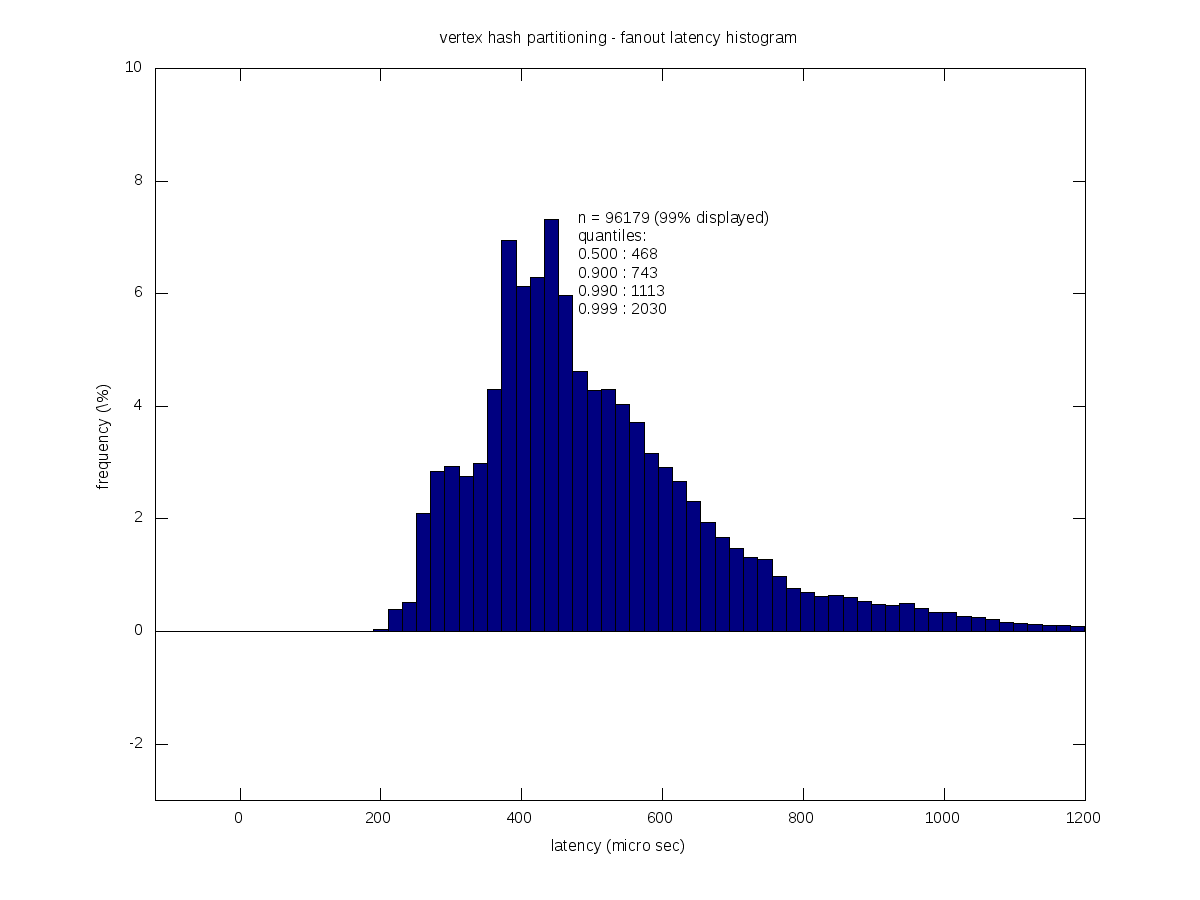
\includegraphics{figures/vertex-fanout.png}}
      \scalebox{0.25}{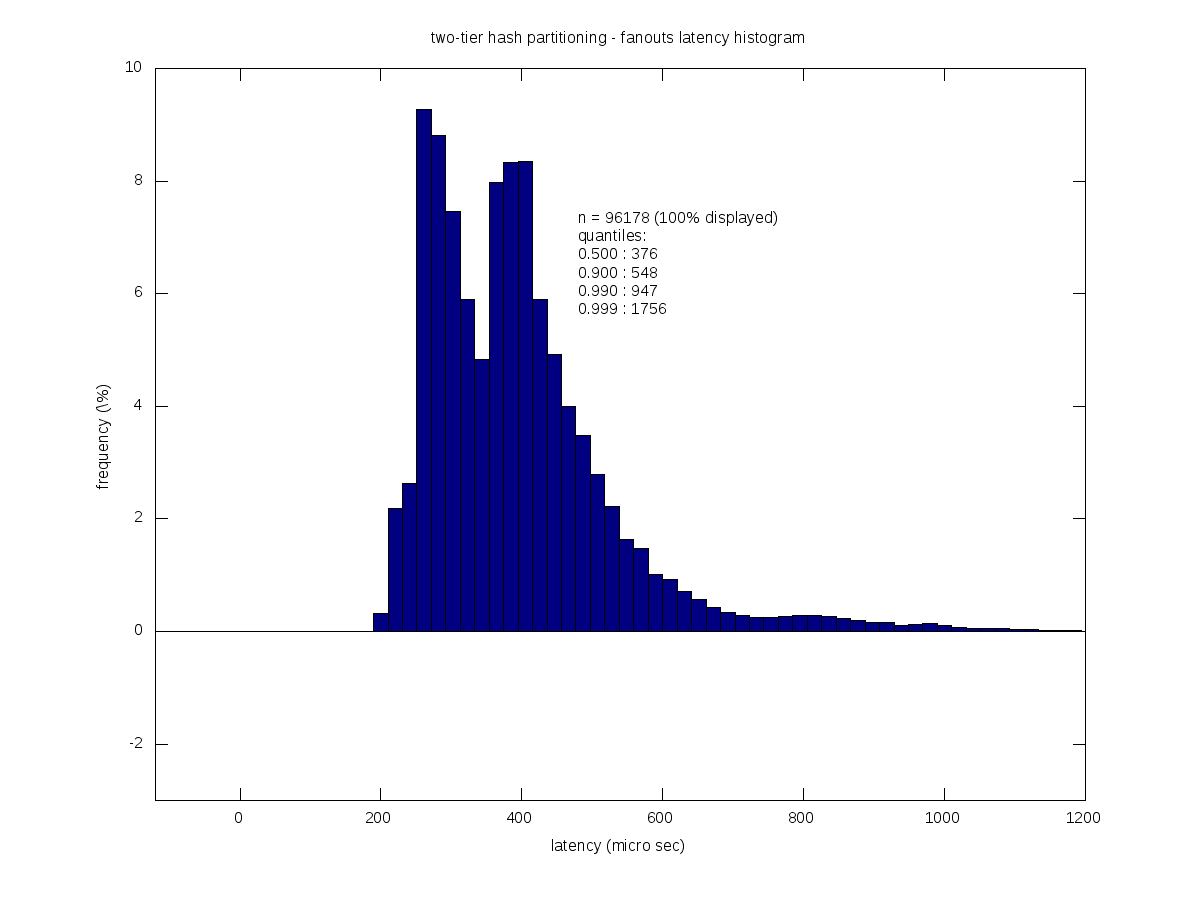
\includegraphics{figures/two-tier2m-fanouts.png}}
      \scalebox{0.25}{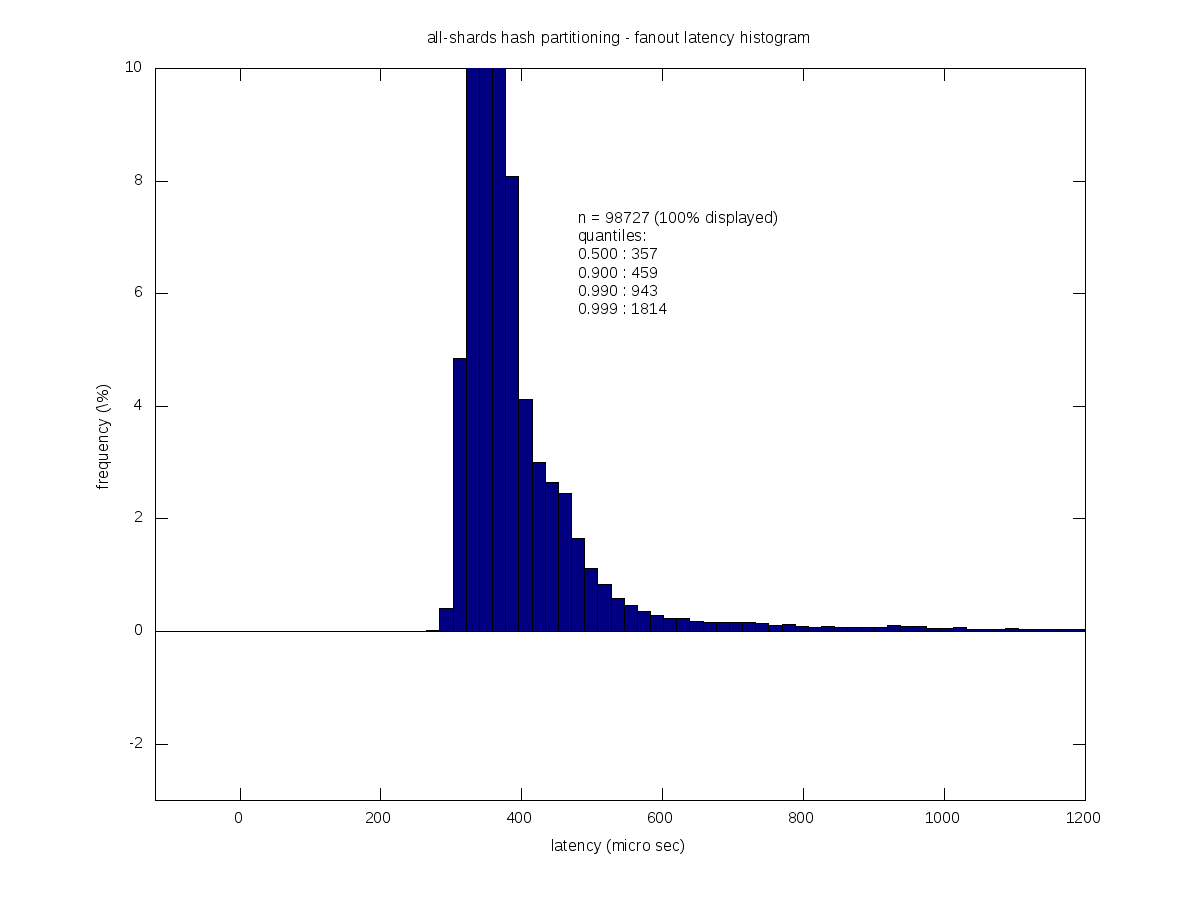
\includegraphics{figures/all-shards-fanout.png}}
  \end{center}
  \caption{Fanout latencies for a) vertex b) upper 2M tier c) all 5 shards hash}
  \label{fig:fanout}

\end{figure}

So when I checked to see performance for 5 way partitioning everything, I got even more improvements for the higher latency ranges. Note latency at higher percentiles is reduced, but increased at lower ones. 


%we never talked about measuring at the 99% percent level .

%percentile05.png  percentile10.png  percentile50.png  percentile99.png for plots of this trend.

\chapter{Optimizing intersection queries}

One motivation for allowing intersections and difference queries to the database is to push filtering as closde to the data as possible. Taking this one step further,  we prefer a query that gets resolved at a single node rather than involve an extra round of communication and external filtering.
I n chapter \ref{chap:background} we described systems that attempt to partition graphs based on its strucure, as well as work such as Schism \cite{schism} that accomplishes this. Ther are two aspects to improving intersection queries. The first is purely algorithmic. We can think of an intersectoin as an equijoin operation, and similar algorithms apply to both. In a distributed data base we attempt to partition tables equally on their frequently joined columns.  This allows easy parallelization of the query: first join locally.  

The optimal algorithm for intersection depends on the relative sizes of the two tables columns. In the case of the graph store, we can think of several possibilities:

%n * m,  n *log m, n logn +  m log m + n + m, n + m O(m) space
%may want to think a bit more about this?
\begin{enumerate}
\item nested loops: $O(nm)$ time, no extra space needed, only small constants costs.
\item sort the entried of the smaller one and then binary search for matches: $O((m + n)\lg{(m)})$ $m$ is the smaller one.
\item construct a hash representation of the smaller set and then query for matches: $O(m + n)$ time, $O(m)$ space, larger constants for constructing the hash.
\item sort- merge: $O(m \lg{m} + n \lg{n})$. If they are already sorted, then we only pay for the  $O(m + n)$ merge.
\end{enumerate}

There are other aspects about this that are important. Like with fanout queries, intersection queries are paged and may not require the full intersection set. They also may require the results in a particular attribute order (different from that of the id set). Moreover, whenever the two fanout sets to intersect are not in the same physical machine, we have to decide which of the two sets moves. 

One effect of limiting the size of the desired result is that the optimal plan may change. If we wish to only get latest common follower, we may want to avoid constructing a full hash. And, especially if the smaller set is very small, we may want to simply loop. There are many optimization techniques that could decide on how to perform the intersection based on the sets involved, and pick a method from the different choices presented.

We are focusing on the relation between partitioning and performance, so we don't try to find  the optimal intersection strategies but instead focus on the effect of reducing the number of distributed queries needed. The main idea we use for optimizing queries is that, just like Schism does for distributed transactions, distributed queries can be improved by using a workload driven approach. If we keep track of frequently intersected pairs and place them together, queries should take less time and the cluster should have a larger maximum throughput, as we consume less resources per query. In the background section we showed that some ids are  intersected a lot more often than others, so, like with fanouts, we

\subsection{Workload driven partitioning}
Imitating the steps from Schism, we partition the graph so that often intersected pairs get placed together. It is tempting for anyone thinking about this problem, including us initially to figure out a way of splitting the social graph  so as to place adjacent nodes together. This kind of partitioning seems natural, since the graph is social it is plausible to infer we should split it via communities  defined by this social structure.  This social graph driven approach has two drawbacks in the case of Twitter infrastructre. The first is the challenge of partitioning the full graph. In the offline case, the graph snapshot was heavy enough that we were not able to get a good result after running METIS for several hours, perhaps using the distributed alternative would speed things up (or maybe not, considering the added communicaton), or perhaps using one of the online algorithms available for this task could make it practical, but either way, the straight forward  approach did not seem to easily scale.   

The second reason this approach is not ideal is that they payoff for such a clustering is not clear either. In the case of Twitter, the user tweet tables  and the user tables are stored separately. Storing a user in the same machine as its followers does not imply more locality in intersection queries unless there is a strong correlation between being followers and intersections.  Since there are no other queries that need locality of this sort, we can avoid using any proxies and use the workload logs themselves to compute which intersections actually happen often.  This is the idea behind the workload driven partitioning. Ideally, this would be an online repartitioning algorithm.  In order to measure its potential effectiveness, on the other hand, I followed the approach suggested in the Schism paper \cite{schism}, and computed a partitioning offline using METIS. The difference is that instead of the social graph driven approach, the graph partitioined by metis is the `operation' graph of a sample. 

We define the operation graph as follows: 

\newtheorem{definition}{Definition}
\begin{definition}
  Follows graph.
  
  Directed graph $G = (V,E)$ where the $V$ are users and an edge $(v,w)$ is in $E$ if and only if $v$ follows $w$.
\end{definition}

\begin{definition}
  Workload graph (for a time interval) 

  Symmetric weighted graph $W_G = (V',E')$  with $V'$ a subset of $V$, with vertex weight for $v$ proportional number of queries involving $v$ in the given interval,  and with edges $\{v, w\}$ in $E'$ with weight $\omega_{vw}$ proportional to the number of intersections involving $v$ and $w$ in the same time interval.
\end{definition}

Both the follows graph $G$  and the corresponding workload graph $W_G$  change over time as edges and vertices are added, but  $W_G$ changes even if $G$ remains the same, depending on the queries received in that time interval.   There are important difference between these graphs. Partitioning $G$ evenly implies that the amount of data stored per node is balanced. Partitioning $G$ minimzing edges means a node is likely to be close to its followers.  On the other hand,  partitioning $W_G$ evenly implies that actual work done across the partitions is even, and that nodes that are often intersected are close together.   Other important differences are that $W_G$ can be small if the time interval is small enough, which provides us a natural way of sampling it by simply sampling the logs.  

In the case of the experiments in this thesis, from the sampled query logs we obtained a graph of 10 million edges (down from 5 billion inthe sampled follows graph). So the partitioning problem is much more tractable.  We did not investigate what the optimal size of the sample is, but this particular sample was enough to improve intersection performance.

(not so for the graph) mention sampling paper.
Importance of adaptive approaches: new stars rise in a matter of days to 
%find a place for this sentence
In effect, because they are different services we can think of the the data tables of users, follows, timelines as vertically partitioned.

% we can mention how the giraph developer argues disconnected nodes may talk to each other as well.
%here we can add synthetic experiment for throughput (but may need to implement descentralized intersections first)

\subsection{Experiments on real data}

We tested the workload driven partitioning strategy on the graph snapshot describe in \ref{chapter:twitterbackground}, using the query logs also described there and a few map-reduce jobs to generate the workload graph and METIS to partition it.  Since the query graph includes only a about 10\%  of the total nodes, we partition the rest of the graph using a hash function and similar to \ref{section:optfanout}.

We then replayed the same log traffic on a database loaded with the same snapshot as above,  One possible effect of this is that performance is better (since we are training on the same data set we are testing), but the experiment is still meaningful because the workload graph is only a proxy for the real workload. 

Results running the intersection queries (for the three techniques) are shown in \ref{fig:intersection}.

\begin{figure}
  \begin{center}
      \scalebox{0.25}{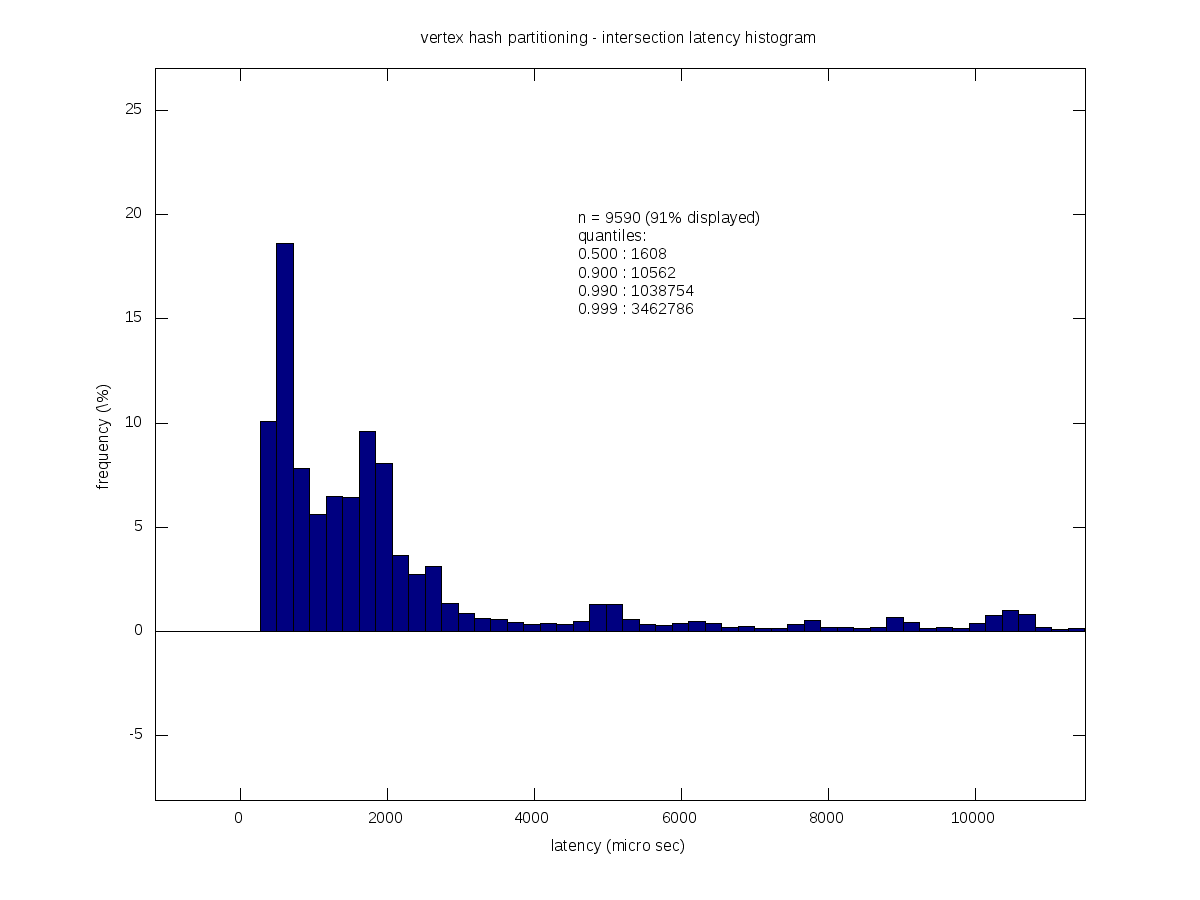
\includegraphics{figures/vertex-intersection.png}}
      \scalebox{0.25}{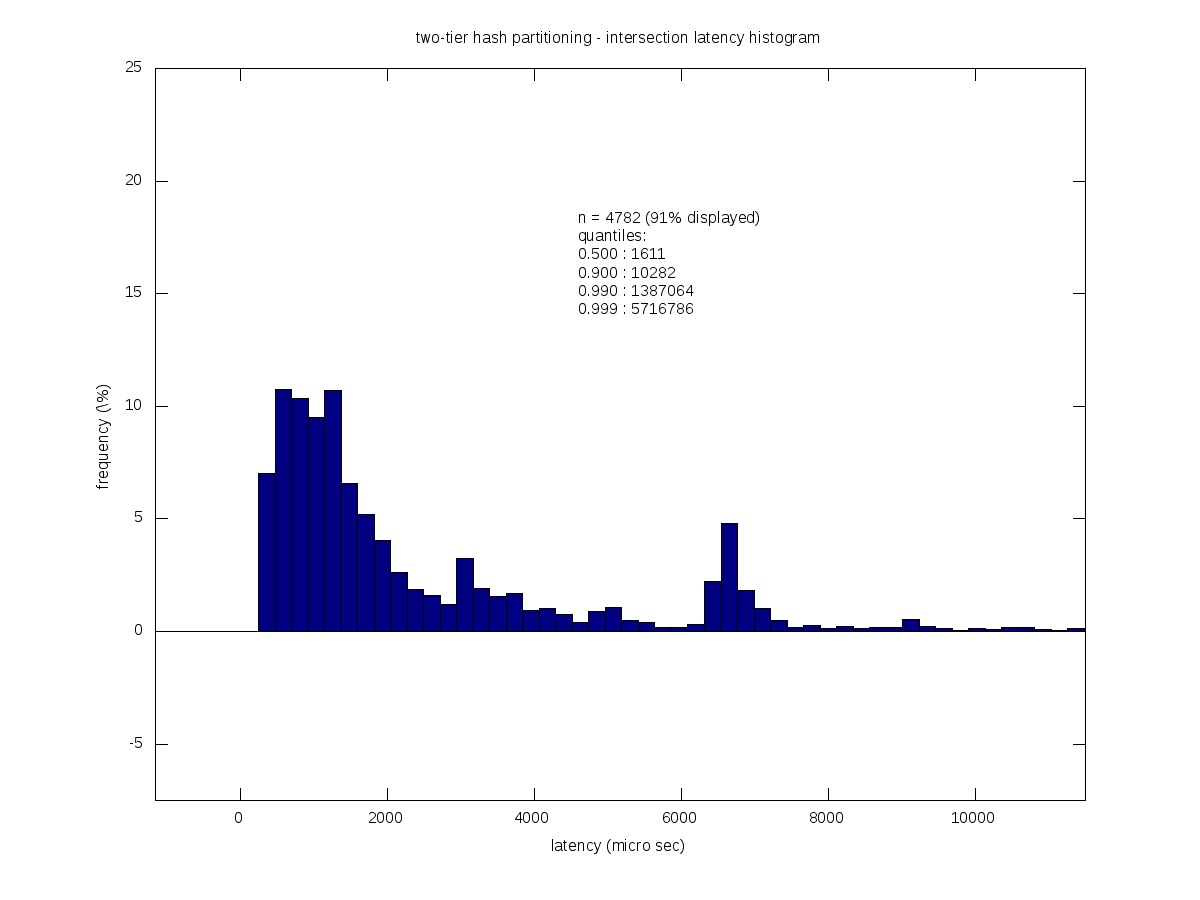
\includegraphics{figures/two-tier2m-intersection.png}}
      \scalebox{0.25}{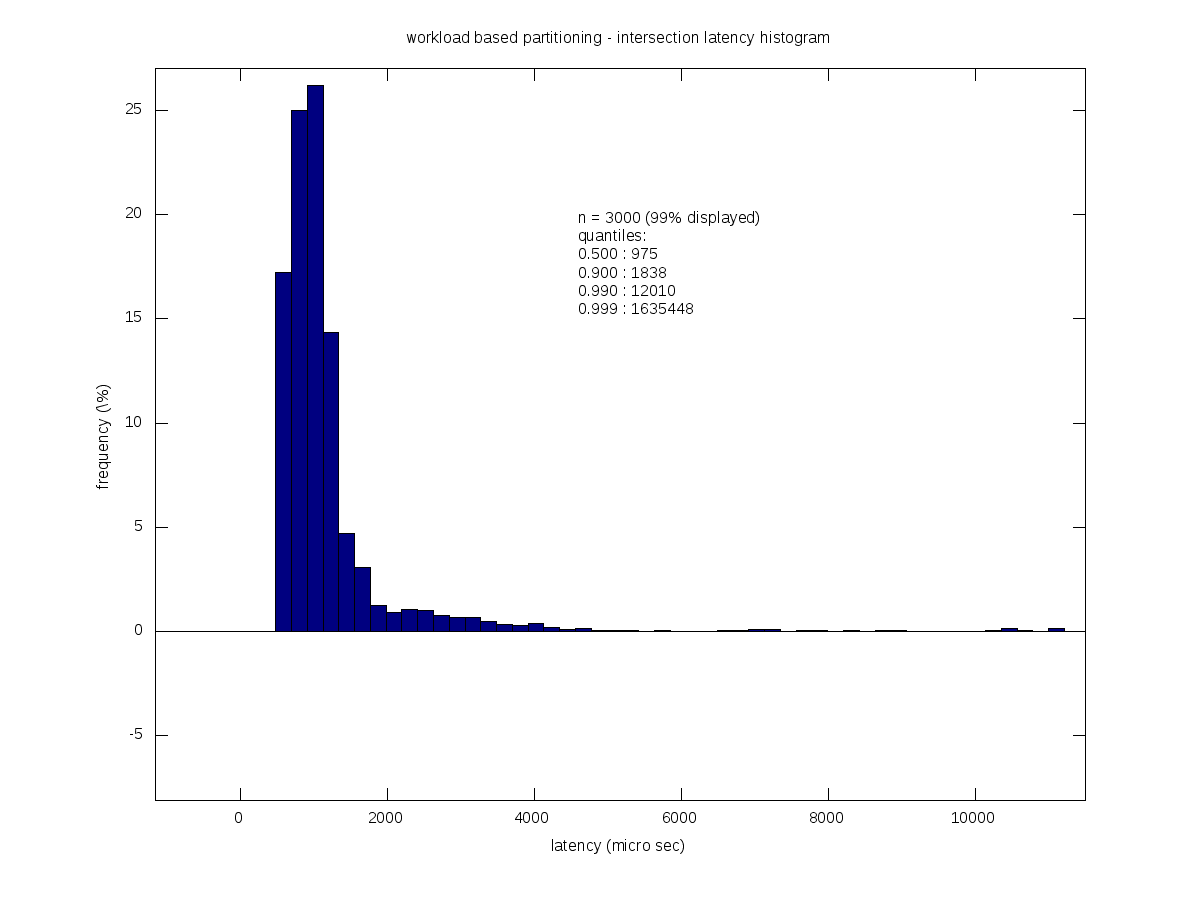
\includegraphics{figures/workload-intersection.png}}
  \end{center}
  \label{fig:intersection}
  \caption{Intersection latencies for a) vertex b) upper 2M tier c) workload based}
\end{figure}


\section{Design}
%information about what I built, (java and pig) goes here. information about results goes here too.

The system was implemented in Java, with a routing layer (the APIServer) that communicated with the data nodes based on its lookup tables via Java RMI calls. Each of the nodes were identical, and held the edge information in memory. For the purposes of this experiment I did not need to support persistence or concurrent modification of the data, since I was measuring read latencies.  I also did not need to support fully dynamic structures, which allowed me to fit enough data using sorted arrays rather than much more space hungry Java maps. These limitations are not fundamental though. Future generations of many Twitter services will be in memory, and disk would be used only to survive. For in memory databases it isn't that necessary to support concurrent writes, because there is no IO bottleneck to use parallelism against. Finally, in a real system the data can be stored compactly by using custom data structures that take much less space, and using systems implement in languages less memory hungry than Java.  Using sorted (static) arrays rather than binary search trees keeps the search time to $O(\lg{n})$. This is helpful to implement the offset logic. It also allows ordered scans of the fanouts that can be merged. Such ordered reads may be less realistic than in a B-tree since they have a lot more locality, but since we only aim to compare the difference between latency at different sizes, it is not a problem.

For benchmark generation I also improved on a ZipfGenerator, which turned out to be a bottleneck whenever I needed to generate numbers zipf distributed in a long interval. Memoization of frequently used internal values helped improve it by far.

The system used in testing the SPAR  heuristic distributes the directory itself into a Hash table.


\chapter{Related and future work}
%here I should bring in some of the background section, and show how it relates 

One interesting topic is analyzing way to make either partitioning adapt to a changing graph. In the case of two-tier hashing we need to react to a node gaining many followers  by repartitioning into several nodes. And, as the node gains more and more followers, keep repartitioning. One option is to use queries as a way to keep a count on followers. Then, use a technique such as consistent hashing to minimize the amount of data moved as we readjust.

For the workload graph based strategy, it is more complicated.  
online partitioning?a
correlation between actual graph and intersection graph?
Neo4j partitioning? how can they do it or do they avoid it? they did not support it at the beginning at least?


